\documentclass[12pt]{article}

\usepackage{times}
\usepackage{amsmath}
\usepackage{latexsym}
\usepackage{fullpage}
\usepackage{graphicx}
\usepackage{amsfonts}

\graphicspath{ {./images/} }

\newcommand{\NOT}{\neg}
\newcommand{\AND}{\wedge}
\newcommand{\OR}{\vee}
\newcommand{\XOR}{\oplus}
\newcommand{\IMPLIES}{\rightarrow}
\newcommand{\IFF}{\leftrightarrow}
\newcommand{\E}{\exists}
\newcommand{\A}{\forall}

\setlength{\parskip}{.1in}

\renewcommand{\baselinestretch}{1.1}

\begin{document}

\begin{center}

{\bf
CSCE 421\\
HW 1\\
Jeffrey Xu\\
09/07/20\\
}

\end{center}

{\bf 1.1.} The gradient of a multi-variate function is a vector of the respective partials of the function. Our given function is shown below:

\begin{center}

$f(x,y)=x^{2}+ln(x)+xy+y^{3}$\\

\end{center}

The gradient vector is as shown below:

\begin{center}

$\begin{bmatrix}
f_{x}\\
f_{y}
\end{bmatrix}
$\\

\end{center}

The gradient values are shown below:

\begin{center}

$f_{x}=2x+x^{-1}+xy+y$\\
\bigskip
$f_{y}=x+3y^{2}$\\
\bigskip
$
\begin{bmatrix}
2x+x^{-1}+xy+y\\
x+3y^{2}
\end{bmatrix}
$
\end{center}

The gradient value for $(1,-1)$ can be computed by plugging those values into the gradient.

\begin{center}

$
\bigtriangledown f(1,-1)=
\begin{bmatrix}
2(1)+1^{-1}+1(-1)+(-1)\\
1+3(-1)^{2}
\end{bmatrix}=
\begin{bmatrix}
1\\
4
\end{bmatrix}
$

\end{center}

{\bf 1.2.} Given the definition of the gradient function, we need to calculate the gradient for the given function below:

\begin{center}

$f(x,y,z)=tanh(x^{3}y^{3})+sin(z)$\\

\end{center}

The partials of the function are shown below:

\begin{center}

$f_{x}=3y^{3}x^{2}sech^{2}(x^{3}y^{3})$\\
\bigskip
$f_{y}=3x^{3}y^{2}sech^{2}(x^{3}y^{3})$\\
\bigskip
$f_{z}=cos(z)$\\
\bigskip
$
\bigtriangledown f=
\begin{bmatrix}
3y^{3}x^{2}sech^{2}(x^{3}y^{3})\\
3x^{3}y^{2}sech^{2}(x^{3}y^{3})\\
cos(z)
\end{bmatrix}
$

\end{center}

The gradient value at $(-1,0,\pi/2)$ is shown below:

\begin{center}

$
\bigtriangledown f(-1,0,\pi/2)=
\begin{bmatrix}
(-1)^{2}(0)^{3}sech^{2}((-1)^{3}(0)^{3})\\
(-1)^{2}(0)^{3}sech^{2}((-1)^{3}(0)^{3})\\
cos(\pi/2)
\end{bmatrix}=
\begin{bmatrix}
0\\
0\\
0
\end{bmatrix}
$\\

\end{center}

{\bf 2.1.} The following matrix multiplication computation is shown below:

\begin{center}

$
\begin{bmatrix}
1 & -1 & 6 & 7\\
9 & 0 & 8 & 1\\
-8 & 5 & 2 & 3\\
10 & 4 & 0 & 1
\end{bmatrix}
\begin{bmatrix}
6 & 2\\
0 & -1\\
-3 & 0\\
11 & 4
\end{bmatrix}=$\\
\bigskip
$
\begin{bmatrix}
1(6)-1(0)-3(6)+7(11) & 1(2)-1(-1)+6(0)+7(4)\\
6(9)+0(0)-3(8)+11 & 9(2)-1(0)+8(0)+4\\
-8(6)+5(0)-3(2)+3(11) & -8(2)-5+2(0)+3(4)\\
10(6)+4(0)-3(0)+11 & 2(10)-4+4\\
\end{bmatrix}=
\begin{bmatrix}
65 & 31\\
41 & 22\\
-21 & -9\\
71 & 20
\end{bmatrix}
$\\

\end{center}

{\bf 2.2.} 
\begin{center}
$
\begin{bmatrix}
10\\
4\\
-1\\
8
\end{bmatrix}
\begin{bmatrix}
7 & 3 & 0 & 1\\
\end{bmatrix}=
\begin{bmatrix}
10(7) & 3(10) & 0(10) & 1(10)\\
4(7) & 3(4) & 0(4) & 1(4)\\
-7 & -3 & 0 & -1\\
8(7) & 3(8) & 0(8) & 1(8)\\
\end{bmatrix}
\begin{bmatrix}
70 & 30 & 0 & 10\\
28 & 12 & 0 & 4\\
-7 & -3 & 0 & -1\\
56 & 24 & 0 & 8
\end{bmatrix}
$

\end{center}

{\bf 2.3} 

\begin{center}
$
\begin{bmatrix}
9 & -3 & 1 & 6\\
\end{bmatrix}
\begin{bmatrix}
-3\\
4\\
-9\\
0\\
\end{bmatrix}=
9(-3)-3(4)+1(-9)+6(0)=-48
$
\end{center}

{\bf 3.1.} We want to calculate the $l_{0}$ norm for each vector given. The two vectors are shown below:

\begin{center}
$
{\bf a}=
\begin{bmatrix}
5\\
0\\
-1\\
4\\
\end{bmatrix}, {\bf b}=
\begin{bmatrix}

7\\
9\\
5\\
2\\
\end{bmatrix}
$\\
\end{center}

The $l_{0}$ norm counts the number of non-zero entries in the vector. For {\bf a}, we can see $l_{0}=3$ and for {\bf b}, $l_{0}=4$. 

{\bf 3.2.} The $l_{1}$ norm is the sum of the absolute values of each element in the vector:

\begin{center}

$l_{1}=\sum_{i=1}^{n}|a_{n}|$\\

\end{center}

For {\bf a}, $l_{1}=|5|+|0|+|-1|+|4|=10$ and for {\bf b}, $l_{1}=|7|+|9|+|5|+|2|=23$.

{\bf 3.3.} The $l_{2}$ norm is simply the square root of the sum of squares of each element:

\begin{center}

$l_{2}=\sqrt{\sum_{i=1}^{n}a_{i}^{2}}$\\

\end{center}

The values of the $l_{2}$ norm for each vector is shown below:

\begin{center}

$l_{2}({\bf a})=\sqrt{5^{2}+0^{2}+(-1)^{2}+4^{2}}=\sqrt{42}$\\
\bigskip
$l_{2}({\bf b})=\sqrt{7^{2}+9^{2}+5^{2}+2^{2}}=\sqrt{159}$\\

\end{center}

{\bf 3.4.} The $l_{\infty}$ norm computes the absolute maximal element in the vector.

\begin{center}

$l_{\infty}=max_{n}|x_{n}|$\\

\end{center}

For {\bf a}, $l_{\infty}=5$ and for {\bf b}, $l_{\infty}=9$. 

{\bf 4.1.} For rolling two dices where each has six faces numbered 1 to 6, the sample space is $\mathbb{Z}[1, 6]*\mathbb{Z}[1,6]$, or the cartesian product of the integers from 1 to 6 with itself. This produces pairs of integers $(1,1), (1,2), (1,3),...,(6,6)$. Note that this notation does specify that the first coordinate denotes the value of the first dice and the second coordinate denotes the value of the second dice. 

{\bf 4.2.} Our sample space has cardinality of 36. Therefore, the probability of any event $X$ can be calculated with the following equation.

\begin{center}

$\mathbb{P}(X)=\dfrac{|X|}{36}$\\

\end{center}

We need to find all the elements of the sample space that satisfy the property that the value of both dices add up to 10. We notice that $(5,5),(6,4),(4,6)$ satisfy this condition. Therefore $\mathbb{P}($Sum of dices equals 10$)=\dfrac{3}{36}=\dfrac{1}{12}$. 

{\bf 4.3.} This problem follows similar logic to the previous question. The elements of $\Omega$ that sum to 6 are $(1,5),(5,1),(2,4),(4,2),(3,3)$. There are 5 elements in this subset, therefore the probability of the sum equalling 6 is $\dfrac{5}{36}$. 

{\bf 5.1.} Recall that the expectation of a continuous random variable can be computed as shown below.

\begin{center}

$E[X]=\displaystyle \int_{-\infty}^{\infty}xp(x)dx$\\

\end{center}

We notice for the Uniform distribution, it is only defined for the interval $[a,b]$. The computation for the expectation of the Uniform distribution is shown below.

\begin{center}

$E[X]=\displaystyle \int_{a}^{b}\dfrac{x}{b-a}dx=\dfrac{1}{b-a}\displaystyle \int_{a}^{b}xdx=$\\
\bigskip
$\dfrac{1}{b-a}[\dfrac{1}{2}x^{2}]_{a}^{b}=\dfrac{1}{2(b-a)}[b^{2}-a^{2}]=\dfrac{(b-a)(b+a)}{2(b-a)}=\dfrac{b+a}{2}$\\

\end{center}

{\bf 5.2.} The standard deviation of a distribution is the square root of the variance of the distribution. The variance of a distribution can be computed using the following equation.

\begin{center}

$Var(X)=E[(X-E[X])^{2}]=E[X^{2}]-E[X]^{2}$\\

\end{center}

The only extra value we need to compute is $E[X^{2}]$. Note, $E[f(x)]=\displaystyle\int f(x)p(x)dx$.

\begin{center}

$E[X^{2}]=\dfrac{1}{b-a}\displaystyle\int_{a}^{b}x^{2}dx=\dfrac{1}{b-a}[\dfrac{1}{3}x^{3}]_{a}^{b}=\dfrac{1}{3(b-a)}[b^{3}-a^{3}]=\dfrac{(b-a)(a^{2}+ab+b^{2})}{3(b-a)}=$\\
\bigskip
$\dfrac{a^{2}+ab+b^{2}}{3}$\\
\bigskip
$Var(X)=\dfrac{a^{2}+ab+b^{2}}{3}-(\dfrac{b+a}{2})^{2}=\dfrac{a^{2}+ab+b^{2}}{3}-\dfrac{b^{2}+2ab+a^{2}}{4}=$\\
\bigskip
$\dfrac{4a^{2}+4ab+4b^{2}}{12}-\dfrac{3b^{2}+6ab+3a^{2}}{12}=\dfrac{b^{2}-2ab+a^{2}}{12}=$\\
\bigskip
$\dfrac{(b-a)^{2}}{12}$\\

\end{center}

Therefore the standard deviation is equal to $\dfrac{b-a}{\sqrt{12}}$. 

{\bf 6.1.} The computation for the accuracy of this detector is shown below.

\begin{center}

$A=\dfrac{37+55}{37+23+45+55}=0.575$\\

\end{center}

{\bf 6.2.} The balanced accuracy weighs each class equally to discourage skewed classification. Let $+1$ denote avocado and $-1$ denote no avocado.

\begin{center}

$A_{+1}=\dfrac{37}{37+23}=0.617$\\
\bigskip
$A_{-1}=\dfrac{55}{45+55}=0.55$\\
\bigskip
$A_{b}=\dfrac{A_{+1}+A_{-1}}{2}=\dfrac{0.617+0.55}{2}=0.5833$\\

\end{center}

{\bf 6.3.} The precision measures the number of true positives detected out of all positives detected.

\begin{center}

$P=\dfrac{TP}{TP+FP}=\dfrac{37}{37+45}=0.45122$\\

\end{center}

{\bf 6.4.} The recall measures the amount of true positives detected out of all positive values.

\begin{center}

$R=\dfrac{TP}{TP+FN}=\dfrac{37}{37+23}=0.617$\\

\end{center}

{\bf 6.5.} The equation for F-measure is shown below.

\begin{center}

$F_{1}=2\dfrac{PR}{P+R}=\dfrac{TP}{TP+0.5(FP+FN)}=\dfrac{37}{37+0.5(45+23)}=0.521$\\

\end{center}

{\bf 7.1.} If the threshold for the ROC is set to 0, then the values for $TP, FP, TN, FN$ are shown below.

\begin{center}

$TP=5$\\
$TN=0$\\
$FP=5$\\
$FN=0$\\

\end{center}

Using these values, the TPR and FPR are calculated to be the following values.

\begin{center}

$TPR=\dfrac{5}{5+0}=1$\\
\bigskip
$FPR=\dfrac{5}{5+0}=1$\\

\end{center}

{\bf 7.2.} The threshold has now increased to $0.25$. This gives us the following values for the confusion matrix.

\begin{center}

$TP=4$\\
$TN=3$\\
$FP=2$\\
$FN=1$\\

\end{center}

These values for the confusion matrix give us the following values for TPR and FPR.

\begin{center}

$TPR=\dfrac{4}{4+1}=\dfrac{4}{5}=0.8$\\
\bigskip
$FPR=\dfrac{2}{2+3}=\dfrac{2}{5}=0.4$\\

\end{center}

{\bf 7.3.} The values for the confusion matrix for a threshold value of 0.5 are shown below.

\begin{center}

$TP=3$\\
$TN=3$\\
$FP=2$\\
$FN=2$\\

\end{center}

The values for TPR and FPR for this threshold value are shown below.

\begin{center}

$TPR=\dfrac{3}{3+2}=\dfrac{3}{5}=0.6$\\
\bigskip
$FPR=\dfrac{2}{2+3}=\dfrac{2}{5}=0.4$\\

\end{center}

{\bf 7.4.} The values for the confusion matrix for a threshold value of 0.75 are shown below.

\begin{center}

$TP=1$\\
$TN=5$\\
$FP=0$\\
$FN=4$\\

\end{center}

The values for TPR and FPR for this threshold value are shown below.

\begin{center}

$TPR=\dfrac{1}{1+4}=\dfrac{1}{5}=0.2$\\
\bigskip
$FPR=\dfrac{0}{0+5}=\dfrac{2}{5}=0$\\

\end{center}

{\bf 7.5.} The values for the confusion matrix for a threshold value of 1 are shown below.

\begin{center}

$TP=0$\\
$TN=5$\\
$FP=0$\\
$FN=5$\\

\end{center}

The values for TPR and FPR for this threshold value are shown below.

\begin{center}

$TPR=\dfrac{0}{0+5}=0$\\
\bigskip
$FPR=\dfrac{0}{0+5}=0$\\

\end{center}

{\bf 7.6.} The plot for the ROC is shown below.

\begin{center}

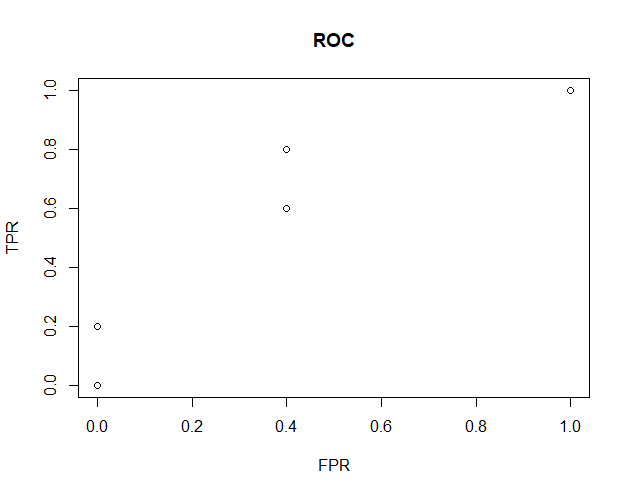
\includegraphics[width=8cm, height=6cm]{ROC_Plot}

\end{center}

To compute this Riemann sum, I will be using a step-size of $0.2$ because the values for each point in the ROC seem to be in steps of $0.2$ and by having step sizes of $0.2$, there would be enough rectangles for a good approximate answer but also not too many rectangles that would result in an inefficient computation time. Looking at the curve, there seems to be two continuous linear lines that compose the ROC curve. I will be using two two lines to determine the heights of the rectangles for the Riemann sums. For values that have two values of TPR for a single value of FPR, I will be only considering the maximal point for the AUROC. The computation for the area of the 5 rectangles is shown below.

\begin{center}

$TPR=0.2+1.5FPR, FPR\in \mathbb{R}[0,0.4]$\\
\bigskip
$TPR=\dfrac{2}{3}+\dfrac{1}{3}FPR, FPR\in \mathbb{R}[0.4,1]$\\
\bigskip
$R_{1}=0.2*h_{1}=0.35*0.2=0.07$\\
\bigskip
$R_{2}=0.2*h_{2}=0.2*0.65=0.13$\\
\bigskip
$R_{3}=0.2*h_{3}=0.2*\dfrac{2}{3}=0.1\bar{33}$\\
\bigskip
$R_{4}=0.2*h_{4}=0.2*0.9=0.18$\\
\bigskip
$R_{5}=0.2*h_{5}=0.2*0.9667=0.19\bar{33}$\\
\bigskip
$\displaystyle \sum_{i=1}^{5}R_{i}=0.7067$\\

\end{center}

\end{document}